% Masterfile

% Laden der Preamble
% This file contains your LaTeX preamble. A preamble is a part of your document where all required packages and macros can be defined. This needs to be done before the \begin{document} command.



% Documentclass:
% Standard LaTeX classes are: article, book, report, slides, and letter. These cover the basis, but are not best. More advanced users might want to try out the KOMA classes or the memoir class. Optional arguments: 10pt. The font size of the main content is set to 10pt with the option between [].

\documentclass[a4paper, 11pt, bibtotocnumbered, liststotocnumbered, toc=listofnumbered, captions=nooneline, fleqn]{scrartcl} 
\usepackage{scrpage2}
%Inhaltsverzeichnis mit im Inhaltsverzeichnis
\setuptoc{toc}{numbered}

%Schriftart
\usepackage{helvet}
\renewcommand{\familydefault}{\sfdefault}

%Deutsches Sprachpaket
\usepackage[ngerman]{babel}
\usepackage[utf8]{inputenc}

%Verbessertes Schriftbild
\usepackage{microtype}

% Geometry:
% The papersize of the document is defined with the geometry package. Here, the size is set to A4 with a4paper. Other possibilities are a5paper, b5paper, letterpaper, legalpaper and executivepaper.
\usepackage[margin=2.5cm]{geometry}
\usepackage[bottom, hang]{footmisc} %Fußnoten nicht einrücken und am Seitenende
\usepackage{longtable} %Tabellen über mehrere Seiten

% AMS math packages:
% Required for proper math display.
\usepackage{amsmath,amsfonts,amsthm}


% Graphicx:
% If you want to include graphics in your document, the graphicx package is required.
\usepackage{graphicx}

% Booktabs:
% The booktabs package is needed for better looking tables. 
\usepackage{booktabs}

% SIunitx:
% The SIunitx package enables the \SI{}{} command. It provides an easy way of working with (SI) units.
\usepackage[decimalsymbol=comma]{siunitx}

% URL:
% Clickable URL's can be made with this package: \url{}.
\usepackage{url}


% Caption:
% For better looking captions. See caption documentation on how to change the format of the captions.
\usepackage{caption}

%Float Package zur Positionierung von Abbildungen
\usepackage{float}
	
%Referenzen Zählweise
\usepackage{chngcntr}
\counterwithin{figure}{section}
\counterwithin{table}{section}
%\counterwithin{equation}{section} Formel durchgehend nummeriert!


%Bild anstelle von Abbildung in der Bildbeschriftung
%\addto\captionsngerman{\renewcommand{\figurename}{Bild}}

%Bildbeschriftung in Fett
\usepackage{caption}
\captionsetup[figure]{labelfont={bf,small}, font={bf,small}}
\captionsetup[table]{labelfont={bf,small}, font={bf,small}}

%Biblatex
%zitieren mit Footcite, Anpassung des Zitierstils gemäß PEM vorgabe
\usepackage[backend=biber, citestyle=authortitle, bibstyle=authortitle, isbn=false, doi=false, url=false, block=space, maxcitenames=2, maxbibnames=99, backref=false, giveninits=true, dashed=false]{biblatex}
\setlength{\bibitemsep}{1em}
\setlength{\bibhang}{2em}
\DefineBibliographyStrings{german}{%
	andothers = {et al.},
}
\DeclareFieldFormat %Klammern um den Kurztitel
[book,article,inbook,incollection,inproceedings,patent,thesis,unpublished,misc,manual]
{citetitle}{\mkbibparens{#1\isdot}}


\renewcommand*{\nametitledelim}{\addspace} %kein Komma hinter dem Autor Namen
\usepackage{xpatch}%Hinzufügen des Erscheinungsjahr in Zitation
\xapptobibmacro{cite}{\setunit{\nametitledelim}\printfield{year}}{}{}

\renewbibmacro*{title}{%
	\ifboolexpr{
		test {\iffieldundef{title}}
		and
		test {\iffieldundef{subtitle}}
	}
	{}
	{\printtext[title]{%
			\printfield[parens]{shorttitle}%
			\setunit{\newline}%
			\printfield[titlecase]{title}%
			\setunit{\subtitlepunct}%
			\printfield[titlecase]{subtitle}}%
		\newunit}%
	\printfield{titleaddon}}

\DeclareFieldFormat %keine Anführungszeichen im Titel
[book,article,inbook,incollection,inproceedings,patent,thesis,unpublished,misc,manual]
{title}{#1\isdot}
\DeclareFieldFormat %keine Klammern beim Jahr
[article,inbook,incollection,inproceedings,patent,thesis,unpublished,misc,manual]
{year}{#1\isdot}

\xpretobibmacro{author}{\mkbibbold\bgroup}{}{}
\xapptobibmacro{author}{\egroup}{}{}

%keine Klammern um Jahr bei Article
\renewbibmacro*{issue+date}{%
	\setunit{\addcomma\space}%
	%
	\iffieldundef{issue}
	{\usebibmacro{date}}
	{\printfield{issue}%
		\setunit*{\addspace}%
		%
		\usebibmacro{date}}
	\newunit}

%Autor-Name Reihenfolge
\DeclareNameAlias{sortname}{last-first}

%Semikolon als Trenner zwischen Autoren und kein "und"
\newcommand*{\bibmultinamedelim}{\addsemicolon\space}
\newcommand*{\bibfinalnamedelim}{\addsemicolon\space}
\AtBeginBibliography{
	\let\multinamedelim\bibmultinamedelim
	\let\finalnamedelim\bibfinalnamedelim
}

\addbibresource{refs/references.bib}

%Array für Tabellen
\usepackage{array}

%Transparent
\usepackage{transparent}

%Abbildung und Tabelle in den Verzeichnissen
\usepackage[titles]{tocloft}
\renewcommand{\cfttabpresnum}{Tabelle }
\renewcommand{\cftfigpresnum}{Abbildung }
\renewcommand{\cftfigaftersnum}{:}
\renewcommand{\cfttabaftersnum}{:}
\settowidth{\cfttabnumwidth}{Tabelle 10 \quad}
\settowidth{\cftfignumwidth}{Abbildung 10 \quad}
%Punkte im Inhaltsverzeichnis bei Section
\renewcommand\cftsecdotsep{\cftdotsep}


%Zeilenabstand definiern
\usepackage{setspace}

%TabularX
\usepackage{tabularx}


%Serifenlose Matheschrift
\usepackage{sfmath}

%Subfigures
\usepackage{subfig}

%Trennung bestimmter Wörter


% Hyperref:
% This package makes all references within your document clickable. By default, these references will become boxed and colored. This is turned back to normal with the \hypersetup command below.
%Dieses Paket sollte möglichst zuletzt geladen werden!
\usepackage{hyperref}
\hypersetup{colorlinks=false,pdfborder=0 0 0}

% Cleveref:
% This package automatically detects the type of reference (equation, table, etc.) when the \cref{} command is used. It then adds a word in front of the reference, i.e. Fig. in front of a reference to a figure. With the \crefname{}{}{} command, these words may be changed.
%Cleverref nach Hyperref Laden!
\usepackage{cleveref}
\crefname{equation}{Gleichung}{Gleichung}
\crefname{figure}{Abbildung}{Abbildungen}	
\crefname{table}{Tabelle}{Tabellen}
\crefname{section}{Kapitel}{Kapitel}
\newcommand{\crefrangeconjunction}{ bis }
\newcommand{\creflastconjunction}{ und }
\newcommand{\crefpairconjunction}{ und }









% Begin des Dokuments
\begin{document}
%Titelseite
\begin{titlepage}
\flushright
\vspace*{-2.3cm}
{\transparent{1}

\includegraphics[scale=0.7]{figs/pem_logo.png}}
\\
\centering
\vspace{0.5cm}
\begin{doublespacing}
	\textbf{Diese Arbeit wurde vorgelegt am Lehrstuhl für Production Engineering of\\ E-Mobility Components (PEM) der RWTH Aachen.}\\
\end{doublespacing}
\vspace{1.5cm}
\textbf{\LARGE Bachelorarbeit}
\\
\flushleft
\vspace{1.7cm}
\Large
\begin{tabular}{lp{10cm}}
	%Name
	\rule[-2ex]{0pt}{2.5ex} Name: & Max Mustermann \\ 
	%Matrikel Nummer
	\rule[-6ex]{0pt}{2.5ex} Matr.-Nr.: & 123456 \\ 
	%Kurzthema
	\rule[-16ex]{0pt}{2.5ex} Thema: & Dies ist der Titel der wissenschaftlichen Arbeit, der Titel kann auch etwas länger sein! \\ 
	%Betreuer
	\rule[-6ex]{0pt}{2.5ex} Betreuender Assistent: & Heinz Mustermann, M.Sc. \\ 
	%1. Prüfer
	\rule[-2ex]{0pt}{2.5ex} 1. Prüfer: & Prof. Dr.-Ing. Peter Mustermann \\ 
	%2. Prüfer
	\rule[-2ex]{0pt}{2.5ex} 2. Prüfer: & Dr.-Ing. Thomas Mustermann \\ 
\end{tabular} 
\\
\vspace{1.2cm}
\hspace{0.15cm}
%Ort und Datum
Aachen, den \today
\\
\vspace{1.4cm}
\hspace{0.15cm}
\begin{minipage}{0.98\textwidth}
	\large
	Inhalt und Ergebnis dieser Arbeit sind ausschließlich zum internen Gebrauch\\ bestimmt. Alle Urheberrechte liegen bei der RWTH Aachen. Ohne ausdrückliche\\ Genehmigung des betreuenden Lehrstuhls ist es nicht gestattet, diese Arbeit oder Teile daraus an Dritte weiterzugeben.
\end{minipage}
\end{titlepage}	
\newpage
\thispagestyle{empty} %leere Seite einfügen
\mbox{}

\newpage

%Überschriften in Kopfzeile inkl. Seitenzahlen
\pagestyle{scrheadings} 
\clearscrheadfoot
\automark[section]{chapter}
\ohead{\pagemark}
\ihead{\headmark}
\setheadsepline{1pt}
\renewcommand{\headfont}{\normalfont \sffamily}
\newcommand{\sectionnumbering}[1] {%
	\setcounter{section}{0}%
	\renewcommand{\thesection}{\csname #1\endcsname{section}}}
%Römische Numerrierung für das Inhaltsverzeichnis und folgende
\renewcommand\thesection{\Roman{section}}

%Inhaltsverzeichnis
\tableofcontents
\pagenumbering{roman} %römische Seitenzahlen
\newpage

%Formelzeichen und Abkürzungen wird über eine Tabelle realisiert
\section{Formelzeichen und Abkürzungen}
\hspace{0.7cm}
\begin{tabularx}{15.1cm}{llX}
	\textbf{Formelzeichen} & \textbf{Einheit} & \textbf{Beschreibung} \\
	\hline \\ [-0.2cm]
	$a(t)$ & $\frac{m}{s^2}$ & Beschleunigungsverlauf \\ [0.1cm]
	$b_{Fzg}$ & $m$ & Fahrzeugbreite \\ [0.1cm]
\end{tabularx}
\vspace{1cm}
\\
\hspace*{0.8cm}
\begin{tabularx}{15.1cm}{lll}
	\textbf{Abkürzung} & \hspace{1.95cm} & \textbf{Beschreibung} \\ %hspace um Breite an obere Tabelle anzupassen!
	\hline \\ [-0.2cm]
	KFZ & & Kraftfahrzeug \\ [0.1cm]
	PEM & & Production Engineering E-Mobility Components \\ [0.1cm]
\end{tabularx}





\newpage

%Abbildungsverzeichnis
\listoffigures
\newpage

%Tabellenverzeichnis
\listoftables
\newpage

%Arabische Numerrierung für die Kapitel
\renewcommand{\theHsection}{arabicsection.\thesection}
\renewcommand\thesection{\arabic{section}}
\setcounter{section}{0}

\section{Einleitung}\label{sec:Einleitung}
%

\newpage
\section{Motivation}\label{sec:Motivation}

Der Transportsektor trägt in der EU mit einem Anteil von ca. 25\% signifikant zu der gesamten Treibhausgasemission (THG) bei. Um die Ziele der EU-Kommission zu erreichen, soll bis 2030 die Anzahl der Fahrzeuge mit konventionellem Antrieb halbiert werden. Bis 2050 soll auf Fahrzeuge mit Benzin- oder Diesel-Motoren komplett verzichtet werden. \\
Eines der Hindernisse für eine Marktdurchdringung der Fahrzeuge mit elektrochemischen Energiespeicher in Form von Lithium-Ionen-Batterien (LIB's) ist die begrenzte Reichweite dieser Fahrzeugklasse\footcite[Vgl.][S.136-146]{Ajanovic2020}.\\
Die Energiedichte von aktuellen LIB's\footcite[Vgl.][S. 11]{Hettesheimer2017} liegt nach Tabelle \ref{tab:Energiedichten} weit unter der von konventionellen Treibstoffen\footcite[Vgl.][]{BeloitEDU2021}, ist jedoch verglichen mit älteren Batterietechnologien erheblich höher\footcite[Vgl.][]{Sollmann2018}. Da auch die Batterie-Aufladezeiten ein Vielfaches der Dauer einer Tankfüllung mit einem Flüssigtreibstoff beträgt, haben Verluste die durch Widerstand oder Abwärme entstehen, zusammen mit Leistung die für das Kühlen bzw. Aufheizen der Batterie aufgewendet werden muss, einen signifikant negativen Effekt auf die Reichweite und Effizienz der Fahrzeuge.\\

\begin{table}[H]
	\caption{Vergleich der Energiedichten von Energieträgern in Fahrzeugen}
	\label{tab:Energiedichten}
	\vspace{0.2cm}	
	\begin{tabularx}{\textwidth}{ |X|X|X|  }
		\toprule[1.5pt]
		\textbf{Typ} & \textbf{Wert} & \textbf{Einheit} \\
		\hline\hline
		Lithium-Ionen-Batterie: & 430 - 800 & Wh/l \\
		\hline
		Nickel-Cadmium-Batterie: & 130 & Wh/l \\
		\hline
		Benzin: & 9700 & Wh/l \\
		\hline
		Diesel: & 10700 & Wh/l \\
		\bottomrule[1.5pt]
	\end{tabularx}		
\end{table}

In der Luftfahrtbranche können durch Lithium-Ionen-Batterien erstmals relevante Reichweiten der Flugzeuge erreicht werden.
Die früheren Konzepte des elektrischen Fliegens waren zwar erfolgreich darin, dass sie das Fliegen mit elektrischem Antrieb ermöglichten, scheiterten jedoch an der geringen Energiedichte verfügbarer Energiespeicher wie Nickel-Cadmium-Batterien und der damit verbundenen möglichen Reichweite\footcite[Vgl.][S. 4]{Hepperle2012}.\\

















%
%%\cref{fig:Blume} zeigt ein Beispiel für eine Abbildung.
%\begin{figure}[H]
%	\flushleft
%	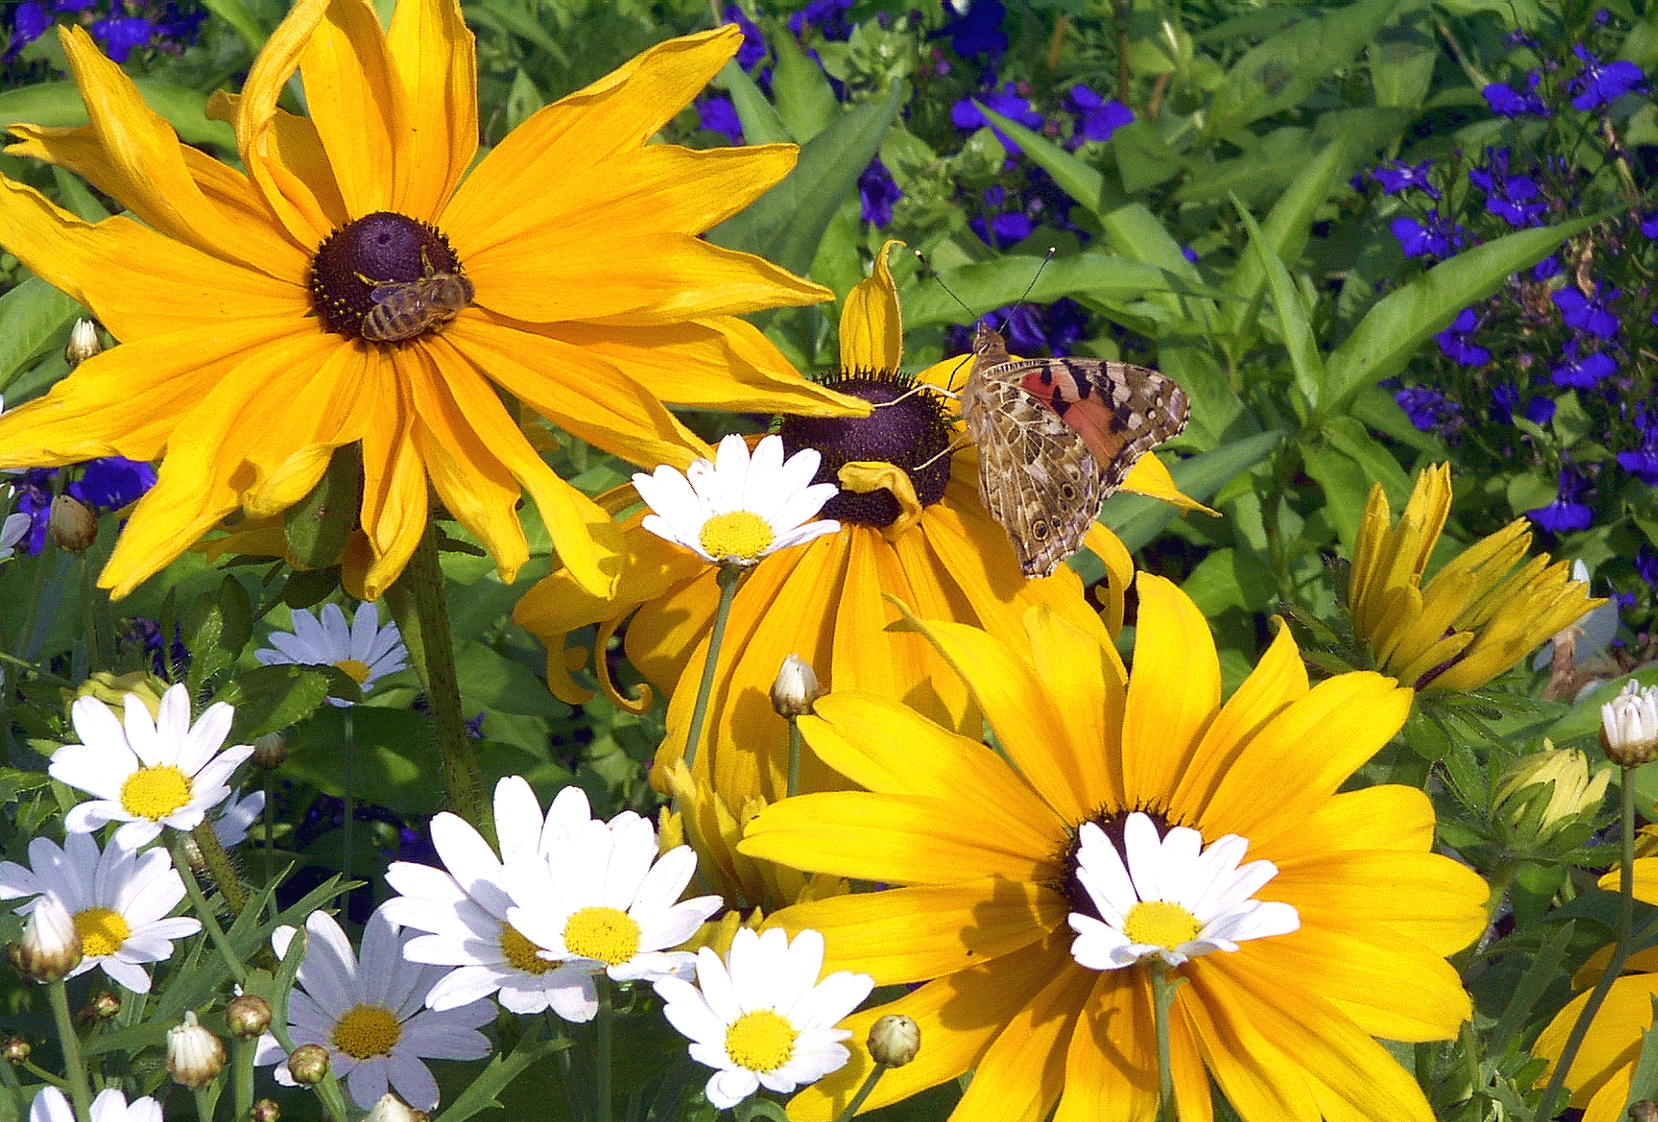
\includegraphics[scale=0.2]{figs/Blume.jpeg}
%	\caption{dies ist eine schöne Blume}
%	\label{fig:Blume} 
%\end{figure}
%\noindent
%\cref{eq:Formel} zeigt ein Beispiel für eine Formel.
%\begin{align}\label{eq:Formel}
%	I = \int_{t_0}^{t_0+n \cdot h} f(t) \hspace{0.1cm} dt
%\end{align}
%\noindent
%\cref{tab:Tabelle} zeig ein Beispiel für eine Tabelle
%\begin{table}[H]
%	\flushleft
%	\caption{Tabelle}
%	\label{tab:Tabelle} 
%	\vspace{0.2cm}
%	\begin{tabularx}{\textwidth}{p{3.5cm}XXXXXXX}
%		\toprule[1.5pt]
%		ABC: & 1 & 2 & 3 \\
%		\midrule[1.0pt]
%		DEF: & 4 & 5 & 6 \\
%		\bottomrule[1.5pt]	
%	\end{tabularx}
%\end{table}
%\noindent
%Zitiert wird mit "footcite". Das sieht dann so %\footcite[Vgl.][S. 456]{PeterPan2017} oder so\footcite[Vgl.][S. 123]{DEF2014} aus.
%%
%\subsection{Unterkapitel 1}\label{subsec:Unterkapitel1}
%%
%%
%\subsection{Unterkapitel 2}\label{subsec:Unterkapitel2}
%%
%\subsubsection{Unterkapitel 2.1}\label{subsec:Unterkapitel2.1}
%%
%
%



\pagenumbering{arabic} %arabische Seitenzahlen
\newpage
\section{Grundlagen und Stand der Technik}\label{sec:GrundlagenUSdT}

\subsection{Lithium-Ionen-Batterietechnologie}\label{subsec:LIB}

In diesem Kapitel wird ein Überblick über die Lithium-Ionen-Batterietechnologie verschafft. Außerdem wird das thermische und elektrische Verhalten der Zellen erläutert. Zuletzt werden noch Alterungsmechanismen und Temperaturabhängigkeiten betrachtet.

\subsubsection*{Aufbau und Funktionsweise}\label{subsec*:LIBAufbau}

Der Begriff Lithium-Ionen-Batterie umfasst viele verschiedene Batterietechnologien, welche alle auf dem gleichen Wirkprinzip beruhen. Analog zu allen anderen Batterietypen besteht eine Lithium-Ionen-Batterie aus dem Elektrolyten, einem Separator und zwei Elektroden.\\
Nach Konvention wird nach den elektrischen Zuständen beim Entladevorgang die negativ geladene Elektrode als Anode und die positiv geladene Elektrode als Kathode bezeichnet.\\

\begin{figure}[H]
	\begin{overpic}[width=12cm]{figs/LIB_Aufbau_Schematic.eps}
			\put(343,180){\mbox{Sauerstoff}}
			\put(343,155){\mbox{Metall}}
			\put(343,130){\mbox{Lithium-Ion}}
			\put(343,105){\mbox{Kohlenstoff(Graphit)}}
			\put(343,80){\mbox{Separator}}
			\put(343,55){\mbox{Entladen}}
			\put(343,30){\mbox{Laden}}
			\put(240,2){\mbox{Anode}}
			\put(25,2){\mbox{Kathode}}
			\put(135,2){\mbox{Elektrolyt}}
			
	\end{overpic}
	
		\caption[Blah]{Aufbau Lithium-Ionen-Batteriezelle in Anlehnung an Ecker u. Sauer 2013}
	
		\label{fig:LithiumIonAufbau}
\end{figure}
%
%
Wie in Abbildung \ref{fig:LithiumIonAufbau} dargestellt, können die Lithium-Ionen durch das Elektrolyt von der Kathode zur Anode oder umgekehrt ?wandern?. \\
Um die Oberfläche für das Einlagern der Ionen möglichst groß zu gestalten, sind die Materialien der beiden Elektroden hochporös. Dies ermöglicht zudem eine hohe Reaktionsrate. \\
Die Kathode einer \textbf{LIB} (Lithium-Ionen-Batterie) besteht meist aus einem Metalloxid, die Anode aus einer Kohlenstoffmodifikation, oftmals Graphit. Für die Bindung der Elektrodenmaterialien wird häufig Polyvinylidenfluorid (PVFD) in verschiedenen Formen verwendet.\\
Diese Materialien werden dann auf einer dünnen Metallfolie aufgetragen. An der Kathode kommt hierfür Aluminium zum Einsatz, an der Anode wird Kupfer verwendet. Diese Metallfolien dienen gleichzeitig als Stromableiter.\\
Der Separator besteht normalerweise aus einem porösen Polymer. Die Bauteile der Batterie, Elektroden und Separator sind in einem Elektrolyt getränkt. Dieses besteht aus Lithiumsalz das in einem organischem Solvat gelöst ist. Das Solvat wird so gewählt, dass es bei den im Betrieb auftretenden Spannungszuständen trotzdem weitgehend stabil ist.\\
Die Bauform der Batteriezellen ist meist einer von drei etablierten Typen, wie in Tabelle \ref{tab:BauformenZelle} dargestellt ist. Bei allen Typen bestehen die Zellen aus mehreren Lagen von Elektroden-Separator-Elektroden-Stapeln, die je nach Typ geschichtet oder gewickelt werden.\\
Das Gehäuse oder das Verpackungsmaterial der Batteriezellen ist ausschließlich aus Metall. Diese Maßnahme dient der Abdichtung der Zelle, da Wassereintritt die Hydrolyse des Leitsalzes $LiPF_{6}$ zu Fluorwasserstoff anstoßen kann. Zudem verhindert das Metall das Diffundieren des Elektrolyten aus der Zelle nach außen\footcite[Vgl.][S.107-117]{Wohrle2013}.\\

\begin{table}[H]
	\caption{Bauformen der Batteriezellen}
	\label{tab:BauformenZelle}
	\vspace{0.2cm}	
	\begin{tabularx}{\textwidth}{ |X|X|X|  }
		\toprule[1.5pt]
		\textbf{Bauform} & \textbf{Geschichtet} & \textbf{Gewickelt} \\
		\hline\hline
		Zylindrisch &  & Ja\\
		\hline
		Prismatisch & Ja & Ja \\
		\hline
		Pouch-Bag & Ja &  \\
		\bottomrule[1.5pt]
	\end{tabularx}		
\end{table}

Je nachdem ob eine höhere Energiedichte oder Leistungsdichte bei den Batteriezellen gewünscht ist, können die Aktivmaterialschichten den Anforderungen entsprechend ausgelegt werden. Bei dünneren Schichten ist die Leistungsdichte, bei gleichzeitig geringerer Energiedichte, höher\footcite[Vlg.\label{Ecker2013}][S.66-67]{Ecker2013}.\\

\subsubsection*{Batterietechnologien}\label{subsub:BatTechnology}

Der größte Unterschied zwischen den LIB-Technologien liegt in der Materialzusammensetzung der Elektroden.\\
Beginnend mit der Lithium-Kobalt-Oxid-Batterie (LCO) von Sony in den 1990er-Jahren, wurden seitdem auch Lithium-Nickel-Oxid- (LNO) oder Lithium-Mangan-Oxid-Batteriezellen (LMO) entwickelt. LNO und LCO weisen beide eine hohe Kapazität auf, LNO besitzt jedoch eine geringe thermische Stabilität und LCO ist aufgrund des Kobaltgehalts in Sachen Kosten, Sicherheit und Umweltverträglichkeit nicht ideal für den Massenmarkt. LMO ist zwar stabil, löst sich jedoch bei Raumtemperatur teilweise im Elektrolyten. \\
Um diese Nachteile auszugleichen wurden beispielsweise die Lithium-Nickel-Mangan-Kobalt-Batteriezelle (NCM) oder die Lithium-Nickel-Kobalt-Aluminium-Batteriezelle (NCA) entwickelt. Eine weitere Variation ist die Batteriezelle mit einer Kathode auf Eisenphosphatbasis (LFP). Diese besitzt verglichen mit den anderen Varianten eine geringere Spannungslage und gravimetrische Energiedichte. Da aber kein Kobalt verbaut wird, besitzt diese Technologie relevante Umweltvorteile.\\
Auch eine alternative Anoden-Technologie, die sogenannte LTO-Zelle (Lithiumtitanat), kommt aktuell auf den Markt. Sie besitzt zwar eine geringere Energiedichte im Vergleich zu anderen Technologien, weist sich jedoch durch eine hohe Leistungsdichte und Lebensdauer aus\footnote{Vgl. Fußnote \ref{Ecker2013}, Ecker und Sauer 2013}.  \\
In der Industrie setzt sich jedoch die NCM-Kathoden-Technologie durch. Zwar sind aktuell in der Transportbranche alle Technologien vertreten, jedoch stellen Produzenten wie Panasonic ihre NCA-Technologie auf die NCM-basierten Zellen um. In der Gigafactory die Panasonic in Zusammenarbeit mit Tesla in Nevada (USA) seit 2017 in Betrieb hat sollen ab 2025 nur noch NCM-Zellen produziert werden. Die Anoden-Technologie wendet weitgehend Graphit basierte Lösungen an.\\
Diese Entwicklung ist auf die Batterie-Roadmaps der OEM-Hersteller zurückzuführen. In diesen Roadmaps stellen Hochenergie-LIB's mit NCM-Basierten Kathoden die aussichtsreichste Wahl was Kosten und Energiedichte angeht dar\footnote{Vgl. Fußnote \ref{cite:Hettesheimer}, Hettenheimer et al. 2017}. \\
Daher wird in dieser Arbeit die NMC-Kathoden-Technologie betrachtet.%ist das wirklich nötig hier??

\subsubsection*{Elektrische Funktionsweise und Kenngrößen der Lithium-Ionen-Batterietechnologie}\label{subsub:ElekChemFunktion}

Während des Entladevorgangs, was dem Auslagern von Lithium aus der negativen Elektrode entspricht, werden Elektronen ausgegeben. Die Lithium-Ionen wandern durch das Elektrolyt und den Separator zur positiven Elektrode und lagern sich dort ein. Gleichzeitig fließen die Elektronen durch die externe Verbindung über einen Verbraucher zur positiven Elektrode wo Aluminium als Stromableiter dient. Beim Laden wird dieser Prozess umgekehrt\footcite[Vgl.\label{cite:Leuthner}][S. 13-19]{Leuthner.2013}.\\
Der Interkalationsprozess der Lithium-Ionen ist nahezu reversibel. Daher tritt unter normalem Gebrauch meist kein Lithium-Plating auf\footcite[Vgl.][S. 265-270]{DAHN1994}.\\
Beim Lithium-Plating setzt sich Lithium an der Anode ab und verringert so die Kapazität der Batterie.\\


Die gebräuchlichen Kenngrößen der Batteriezelle sind meist die nominale Kapazität, elektrische Energie und Leistung. \\
Die Kapazität ist die Menge an elektrischer Ladung, welche von einer Leistungsquelle während der Entladung geliefert werden kann. Sie wird primär von dem Entladestrom, der Temperatur, der Entladeschlussspannung und der Art und Menge der Aktivmaterialien auf den Elektroden beeinflusst. Die Einheit ist [\textbf{Ah}].\\
Die Energie einer Batteriezelle berechent sich aus der Kapazität und der mittleren Entladespannung und wird in der Einheit [\textbf{Wh}] angegeben. Die Energiedichte bezieht sich auf das Volumen der Batterie und wird in [\textbf{Wh/l}] gerechnet. Die spezifische Energiedichte referenziert die Masse der Batterie und wird dementsprechend in [\textbf{Wh/kg}] angegeben.\\
Um die Leistung zu berechnen wird der Strom mit der Spannung multipliziert, was die Einheit Watt [\textbf{W}] ergibt. Durch den nahezu reversiblen Prozess ist der Wirkungsgrad von Lithium-Ionen-Batterien sehr hoch. Dieser ist nach Gleichung \ref{gl:WirkungsgradLIB} definiert als die Energie die bei der Entladung frei wird geteilt durch die Energie, die beim Laden aufgewendet wird\footnote{Vgl. Fußnote \ref{cite:Leuthner}, Leuthner 2013}.\\

\begin{equation}
	\mbox{Wirkungsgrad} = \frac{Entladeenerige}{Ladeenergie}
	\label{gl:WirkungsgradLIB}
\end{equation}


\subsubsection*{Bauformen der Lithium-Ionen-Batterien}\label{subsub:BauformenLIB}

Wie in Tabelle \ref{tab:BauformenZelle} dargestellt, gibt es drei Bauformen von Lithium-Ionen-Batterien. Da in dieser Arbeit nur die zylindrische und prismatische Bauform relevant ist, werden nur sie hier behandelt.\\
Die zylindrische Zelle besitzt gewickelte Elektroden-Separator-Elektroden-Paare. Analog zu einer klassischen AA-Batterie sind die positiven und negativen Anschlüsse auf jeweils einer der beiden Stirnseiten angebracht. In der konventionellen Batteriezelle wird der Strom durch ein sogenanntes $"Tab"$ aus den Kathoden-Anoden-Paaren entnommen. Der $Tab$ der Kathode oder Anode ist demnach an einer Stelle der Elektrode angebracht. Dadurch muss der Strom zum Teil große Distanzen zurücklegen um über die $Tab$-Verbindung zum elektrischen Leitstück am Ende der Batteriehülle, oder $Can$, zu gelangen. In Kapitel \ref{} wird dieser Prozess näher erläutert.\\ %%%%%%%%%%%%%%%%%%%%%%%% HIER NOCH REFERENCE EINFUEGEN!!!!!!!%%%%
Die Bauform der zylindrischen Zelle wird häufig durch ein Zahlenkürzel angegeben, bei dem die ersten beiden Ziffern den Durchmesser in [mm] vorgeben. Die nächsten beiden Ziffern stehen für die Zellhöhe, wieder in [mm]. Die letzte Ziffer ist eine 0 und schließt die Zahl ab. Zum Beispiel ist eine häufige Bauform die 18650er Zelle mit einem Durchmesser von 18 mm und einer Höhe von 65 mm. Auch viel verwendet werden die 26650er- und die 21700er-Zellgrößen\footcite[Vgl.][]{LionKnowledge2021Zylind}.\\


\begin{figure}[!h]
	\begin{center}
		\begin{overpic}[width=12cm]{figs/Prismatische_und_Zylindrische_Zelle.eps}
		\put(20,250){\mbox{Zylindrische Zelle}}
		\put(225,250){\mbox{Prismatische Zelle}}
		
		\end{overpic}
	\end{center}
	
	
	\caption[Blah]{Prismatische und zylindrische Batteriezelle in Anlehnung an Ecker u. Sauer 2013}
	
	\label{fig:PrismaZylindZelle}
\end{figure}

Der Aufbau der prismatischen Zelle (siehe Abbildung \ref{fig:PrismaZylindZelle}) ist relativ einfach. \\
In diesem Bauformat werden gewickelte oder geschichtete Elektrodenpaare verwendet. Die Spannungs-, bzw. Stromentnahme erfolgt analog zu der konventionellen zylindrischen Batterie-\newline zelle über $"Tabs"$ und wird über an der Kopfseite der Batteriezelle angebrachte Anschlüsse entnommen.\\
Die Größe der prismatischen Zellen variiert stark und wird je nach Anwendungsfall bestimmt\footcite[Vgl.][]{LionKnowledge2021Prisma}. 


\subsubsection*{Alterungsmechanismen}\label{subsub:alterung}

Die Temperaturgradienten die sich beim Benutzen der Batterie in der Zelle ausbilden, können auch Alterungsgradienten hervorrufen. Hinzu kommt, dass starke Temperaturgradienten, die z.B. während hoher C-Raten auftreten, Verformungen der Elektrodenwickel induzieren können\footcite[Vgl.][S.921-927]{Waldmann2015}.\\
Es ist also zu Schlussfolgern, dass eine homogene Temperaturverteilung innerhalb der Zelle von Vorteil ist.
Im weiteren werden drei häufig auftretende Alterungsmechanismen erläutert.\\
Beim Lithium-Plating setzen sich Lithium-Ionen auf der Trennschicht, oder ``Solid Electrolyte Interface" (SEI), zwischen Elektrode und Elektrolyt durch irreversible chemische Reaktionen ab. Diese Ablagerungen verdicken die Trennschicht, was zu einem Anstieg des Stofftransportwiderstands und dadurch zu einem Anstieg des ohm'schen Wiederstands führt. Da die Konzentration der Lithium-Ionen im Elektrolyt auch abnimmt, kommt es außerdem zu einem Kapazitätsverlust.\\
Alterung kann außerdem durch mechanische Spannungen ausgelöst werden. Diese entstehen, wenn Lithium-Ionen sich in die Aktivmaterialien einlagern. Die Spannung innerhalb der Partikel kann hierbei zur Rissbildung führen. Durch die Risse sind die Teile des Aktivmaterials nicht mehr elektrisch angebunden und werden als ``Dead-Lithium`` bezeichnet.\\
Der letzte hier behandelte Alterungsvorgang entsteht aus Dehnvorgängen bei der Lithium-Einlagerung. Diese Belastung kann den Leitruß, einen speziellen Kohlenstoffleiter der Leitpfade zwischen Stromableitern und Partikeln bereitstellt, auftrennen. Dadurch sind die Aktivmaterialpartikel nicht mehr mit dem Stromableiter verbunden. Dieser Alterungsvorgang kann sowohl an Kathode, als auch an der Anode auftreten.\footnote{Vgl. Fußnote \ref{cite:Leuthner}, Leuthner 2013}\\

\subsubsection*{Wärmeentwicklung und Temperatureinfluss auf die Batteriezelle}\label{subsub:waermeundtemperatur}

Die Leistung von LIB's hängt stark von der Zelltemperatur ab. \\
Mit sinkender Temperatur steigt der innere Widerstand der Zelle und die verfügbare Kapazität nimmt ab. Dies führt zu verminderter abnehmbarer Energie und geringerer maximaler Leistung. Bei hoher Zelltemperatur kann jedoch die Sicherheit der Batteriezelle nicht mehr gewährleistet werden und es finden Alterungsprozesse statt. Die Zelltemperatur ist hierbei von der Außentemperatur und der Wärmeentstehung beim Laden bzw. Entladen der Batterie abhängig.\footcite[Vgl.\label{cite:Liu}][S.1001-1010]{Liu2014} \\
Liu et al. stellen Gleichung \ref{gl:cycleheatgeneration} für die Berechnung der Wärmegeneration in der Batteriezelle während der Ladezyklen auf.


\begin{equation}\label{gl:cycleheatgeneration}
		\dot{Q} = I \cdot (U_{OCV} - U_{t}) 
		- I \cdot T \frac{\partial U_{OVC}}{\partial T} 
		- \sum_{i}^{ } \bigtriangleup H_{i}^{avg}r_{i}
		- \int \sum_{i}^{ } (\overline{H_{j}} - \overline{H_{j}^{avg}})	\cdot \frac{\partial c_{j}}{\partial t} dv
\end{equation}

\begin{table}[h!]
	\caption{Variablen aus Gleichung \ref{gl:cycleheatgeneration}}
	\label{tab:variablenheatgeneration}
	\vspace{0.2cm}	
	\begin{tabularx}{\textwidth}{ |X|X|  }
		\toprule[1.5pt]
		\textbf{Nummer} & \textbf{Beschreibung} \\
		\hline\hline
		$\dot{Q}$ & Wärmeentstehungsrate \\
		\hline
		$I$ & Batteriestrom\\
		\hline
		$U_{t}$ & Klemmenspannung der Batterie\\
		\hline
		$U_{OCV}$ & Leerlaufspannung der Batterie\\
		\hline
		$T$ & Batterietemperatur\\
		\hline
		$\bigtriangleup H_{i}$ & Entropieänderung der $i$-ten Reaktion \\
		\hline
		$r_{i}$ & Reaktionsrate der $i$-ten Reaktion\\
		\hline
		$\overline{H_{j}}$ & Molare Entropie des $j$-ten Teils der Batterie\\
		\hline
		$c_{j}$ & Ionenkonzentration im $j$-ten Teil\\
		\hline
		$v$ & Volumen\\
		\hline
		$X^{avg}$ & Entspricht der Durchschnittskonzentration in einem Teilvolumen\\
		\bottomrule[1.5pt]
	\end{tabularx}		
\end{table}

Der erste Term von Gleichung \ref{gl:cycleheatgeneration} auf der rechte Seite entspricht der ohm'schen Wärmeentstehung, kurz $\dot{Q}_{jou}$. Der zweite Term ist die reversible Entropiewärme oder Reaktionswärme, $\dot{Q}_{re}$. Der dritte Term ist die Wärme aus Nebenreaktionen, $\dot{Q}_{sr}$. Dieser beschreibt die Alterung der Batteriezelle und kann für wenige Testzyklen vernachlässigt werden\footcite[Vgl.][]{Forgez2010}. Der letzte Term, $\dot{Q}_{mix}$, entspricht der Wärme im Mischprozess der Batterie. Die Mischprozesswärme entsteht durch die Bildung und Entspannung von Zellkonzentrationsgradienten. Für dynamische Belastungsprofile ist sie daher signifikant und kann nicht vernachlässigt werden\footcite[Vgl.][]{Thomas2003}. \\
Zusammengefasst verkürzt sich Gleichung \ref{gl:cycleheatgeneration} demnach zu Gleichung \ref{gl:cycleheatshort}.

\begin{equation}\label{gl:cycleheatshort}
	\dot{Q} = \dot{Q}_{jou} + \dot{Q}_{sr} + \dot{Q}_{mix}
\end{equation}

Nach Gleichung \ref{gl:cycleheatgeneration} ist die ohm'sche Wärme von dem Stromfluss und der Überpotential abhängig. Das Überpotential entsteht durch den Potentialverlust durch einen erhöhten inneren Widerstand der Batteriezelle.\\
Folgend kann der innere Zellwiderstand $R_{in}$ nach Gleichung \ref{gl:innererWiderstand} definiert werden.\footnote{Vgl. Fußnote \ref{cite:Liu}, Lui et al. 2014}

\begin{equation}\label{gl:innererWiderstand}
	R_{in} = \frac{U_{OCV} - U_{t}}{I}
\end{equation}

Der innere Widerstand einer Lithium-Ionen-Batterie wird durch das State-Of-Charge (SOC), die Zellalterung und die Zelltemperatur beeinflusst. Im Allgemeinen sind die Kausalitäten bereits bekannt. Der Widerstand nimmt mit fallender Zelltemperatur zu. Außerdem variiert er mit dem SOC und steigt über die Lebensdauer mit dem Auftreten von Alterungsmechanismen.\footcite[Vgl.][]{Andre.2011}$\;$\footcite[Vgl.][]{Ecker.2012}\\
Interessant ist auch, dass der Ladewiderstand kleiner als der Entladewiderstand ist. Daher wird während dem Ladeprozess weniger ohm'sche Wärme produziert als beim Entladeprozess. Andererseits beeinflusst die Zelldegradation den Ladewiderstand mehr als den Entladewiderstand, wodurch Alterungseffekte beim Berechnen der Wärmeentstehung während Ladezyklen signifikant sind.\\
Bei der Reaktionswärme ist der dominierende Einfluss nach Liu et al. das SOC. In manchen SOC-Bereichen sollten Alterungseffekte berücksichtigt werden und der Temperatureinfluss ist nicht vernachlässigbar.\footnote{Vgl. Fußnote \ref{cite:Liu}, Liu et al. 2014}

\newpage
\subsection{Das Tesla-Patent}

Im Folgenden wird das Patent von Tesla für eine innovative thermische und elektrische Anbindung des Elektrodenwickels an das Batteriegehäuse für die Leistungsabnahme behandelt.\\
Das Patent wurde von Tesla Inc. mit den Erfindern Tsuruta et al am 4. November 2019 eingereicht und am 7. Mai 2020 unter der $Publishing\,No.$ \textbf{US 2020/0144676 A1} veröffentlicht\footcite[Vgl.\label{cite:TeslaPatent}][]{TsurutaTesla2020}.\\
Der Abstract der Veröffentlichung fasst die Erfindung, bei der es sich um eine zylindrische Zelle handelt, wie folgt zusammen: \\
``Eine Zelle eines Energiespeichergeräts mit mindestens einer Elektrode die ohne $Tab$ konstruiert wird und Herstellungsmethoden dieser."\\

In der konventionellen Batteriezelle, ob zylindrisch oder prismatisch, werden die Kathode und Anode mit den positiven und negativen Anschlüssen mithilfe von $Tabs$ verbunden (Beispiel $Tab$ siehe Abbildung \ref{fig:JellyRoll} mit Tabelle \ref{tab:BeschriftungJellyRoll}). \\
Diese $Tabs$ dienen als sogenannte ``Current collectors", d.h. durch sie fließt der gesamte Strom den die Batteriezelle abgibt oder aufnimmt. \\
Da der Widerstand nach Gleichung \ref{gl:WiderstandElektrisch} von der Dichte des Materials ($\rho$), der Länge die der Strom zurücklegt (l) und der Fläche (A) durch den er fließt abhängt, haben Tsuruta et al in ihrem Patent die zurückgelegte Distanz reduziert und die Fläche vergrößert um den Widerstand zu verringern\footnote{Vgl. Fußnote \ref{cite:TeslaPatent}, Tsuruta et al. 2020}.
\begin{equation}
	R = \rho \cdot \frac{l}{A}
	\label{gl:WiderstandElektrisch}
\end{equation}

Im konventionellen Design sind die $Tabs$ entweder in der Mitte oder an einem Ende der Elektrode angebracht. Daher muss der Strom zuerst mindestens die Hälfte, beim $Tab$ am Ende der Elektrode die gesamte Länge der Elektrode zurücklegen. \\
Bei dem innovativen Entwurf ist die maximale Distanz die der Strom zurücklegen muss die Höhe der Elektrode. Abhängend vom Batteriezellenformfaktor entspricht die Höhe der Elektrode typischerweise $5\percent-20\percent$ der Länge. Es folgt, dass der ohm'sche Widerstand des elektrochemischen Zyklus' des innovativen Konzepts 5- bis 20-Mal kleiner ist als der Widerstand des konventionellen Konzepts\footnote{Vgl. Fußnote \ref{cite:TeslaPatent}, Tsuruta et al. 2020}.\\
Ein weiterer Effekt der durch das innovative Konzept hervorgerufen wird ist, dass signifikant weniger Stromabweichungen (Checken mit Jonas) (Stromverteilung auf der Elektrode) auftreten. Stromabweichung ist das Phänomen bei dem manche Elektrodenregionen mehr oder weniger Strom als andere Regionen auf der selben Elektrode während der Zyklendauer leiten.\\
Nach Ohm fließt Strom bevorzugt entlang der Strecke mit dem geringsten Widerstand (siehe Gleichung \ref{gl:OhmsLaw}). In dem konventionellen Design entspricht dies dem Bereich auf der Elektrode nahe des $Tabs$. Die auftretenden Stromabweichungen sind unerwünscht, da es zur Entstehung von lokalen ``Elektroden-Hotspots`` führt. Hier treten Spannungsüberhöhungen auf, welche chemische Reaktionen hervorrufen die die Lebensdauer der Zelle reduzieren. Ein Beispiel einer solchen Reaktion ist Lithium-Plating\footnote{Vgl. Fußnote \ref{cite:TeslaPatent}, Tsuruta et al. 2020}.
\begin{equation}
	I = \frac{V}{R}
	\label{gl:OhmsLaw}
\end{equation}

Die innovativen Konzepte bieten laut Patentschrift auch verbesserte Wärmeentstehungs- und Wärmeübertragungseigenschaften.\\
Nach Gleichung \ref{gl:HeatResistance} ist die ohm'sche Erhitzung in [\textbf{W}] abhängig von dem Strom und dem Widerstand. 
\begin{equation}
	 P \approx I^{2} \cdot R
	 \label{gl:HeatResistance}
\end{equation}

Da der Widerstand \textbf{R} zwischen 5 und 20 mal kleiner ist als beim konventionelle Entwurf ist zu erwarten, dass beim innovativen Design die ohm'sche Wärmeproduktion signifikant reduziert ist.\\
Die trotz der Maßnahmen entstehende Wärme kann effizienter abgeführt werden.
\begin{equation}
	\dot{Q} = \frac{k\cdot A\cdot (T_{2} - T_{1})}{d}
	\label{gl:HeatTransferEquation}
\end{equation}

Gleichung \ref{gl:HeatTransferEquation} beschreibt den Wärmetransport durch ein wärmeleitendes Medium. \.{Q} ist der Wärmestrom in [\textbf{$\frac{Joule}{Sekunde}$}]. k ist der Wärmeleitkoeffizient des Materials in [\textbf{$\frac{W}{mK}$}].
Die Fläche A in [\textbf{$m^{2}$}] und die Distanz d in [\textbf{$m$}] sind die geometrischen Dimensionen über die der Transfer stattfindet. Der Term $(T_{2}-T_{1})$ entspricht der Temperaturdifferenz über d.\\
In konventionellen Batteriezellen wird die Kontaktfläche zwischen Elektrode und Batteriegehäuse vom $Tab$ realisiert. Beim innovativen Entwurf entspricht der Kontakt zwischen Elektrode und Gehäuse der gesamten Elektrodenlänge. Der Bereich (\textbf{1}) der Elektrode in Abbildung \ref{fig:JellyRoll} befindet sich im Kontakt mit dem Gehäuse und nimmt effektiv $100\percent$ des Durchmessers des Batterie-\newline zylinders ein. Die signifikant größere Kontaktfläche ermöglicht erhöhte Wärmeleitung und dadurch eine optimierte Temperaturkontrolle der Batteriezelle\footnote{Vgl. Fußnote \ref{cite:TeslaPatent}, Tsuruta et al. 2020}.\\

\subsubsection*{Inhalte des Patents}\label{subsub:PatentContents}

In der Patentschrift wird auch auf mögliche Herstellungsvorgänge für die Elektrodenbeschichtung eingegangen. Da diese Arbeit sich mit den physikalischen Vorgängen in der Batteriezelle auseinandersetzt wird die Produktion an dieser Stelle nicht weiter behandelt. Bei Interesse an der Produktion wird die Patentschrift als weiterführende Literatur empfohlen.\\
Es werden verschiedene Konfigurationen der Elektrodenwickel beschrieben. In Abbildung \ref{fig:JellyRoll} ist ein Beispiel für eine ``Jelly-Roll`` zu sehen. \\
Die Kathode oder Anode (\textbf{3}) wird mit dem Aktivmaterial beschichtet. Dabei kann der leitende Teil an dem unteren Ende der Elektrode (\textbf{1}) durch eine isolierende Schicht (\textbf{2}) von dem Aktivmaterial getrennt werden. Diese Schicht ist in manchen Konfigurationen des Patents jedoch nicht vorhanden.\\
Zwischen die beiden Elektroden wird eine Trennschicht eingebracht (\textbf{4}). Da die Elektroden gewickelt werden, wird nach der Anode oder Kathode (\textbf{5}) eine weitere, äußere Trennschicht (\textbf{6}) eingebracht. Diese 4 Schichten werden dann um eine zentrale Achse \textbf{AA'} gewickelt. (\textbf{7}) zeigt das $Tab$ der Anode oder Kathode, welches mit der oberen Seite des Gehäuses verbunden wird.\\
\begin{figure}[H]
	\begin{center}
		\begin{overpic}[width=14 cm]{figs/JellyRollTeslaPatent.eps}
			\put(0,-2){(\textbf{1})}
			\put(-9,27){(\textbf{2})}
			\put(-11,132){(\textbf{3})}
			\put(-14,220){(\textbf{4})}
			\put(-8,270){(\textbf{5})}
			\put(35,302){(\textbf{6})}
			\put(392,232){(\textbf{7})}
			\put(292,270){\textbf{AA'}}
		\end{overpic}
	\end{center}
	
	
	\caption[Blah]{Aufbau des Elektrodenwickels in der zylindrischen Zelle in Anlehnung an Tesla Patent, Tsuruta et al. 2020}
	
	\label{fig:JellyRoll}
\end{figure}

\begin{table}[h!]
	\caption{Beschriftung von Abbildung \ref{fig:JellyRoll}}
	\label{tab:BeschriftungJellyRoll}
	\vspace{0.2cm}	
	\begin{tabularx}{\textwidth}{ |X|X|  }
		\toprule[1.5pt]
		\textbf{Nummer} & \textbf{Beschreibung} \\
		\hline\hline
		(1) & Leitfähiges Material \\
		\hline
		(2) & Isolierendes Material\\
		\hline
		(3) & Kathode/Anode\\
		\hline
		(4) & Innere Trennschicht\\
		\hline
		(5) & Anode/Kathode\\
		\hline
		(6) & Äußere Trennschicht\\
		\hline
		(7) & $Tab$\\
		\bottomrule[1.5pt]
	\end{tabularx}		
\end{table}

\subsubsection*{Der Kontakt zwischen Elektrodenwickel und Cap}\label{subsub:JellyrollCapContact}

Damit der leitende Teil der Elektrode Kontakt zum entsprechenden Pol des Batteriegehäuses hat, wird ein Ende des Batteriezylinders mit einer $Cap$ versehen. Das $Cap$ besteht aus einem leitenden Material, zum Beispiel einer Nickel-Legierung\footnote{Vgl. Fußnote \ref{cite:TeslaPatent} S. 1, Tsuruta et al. 2020}.\\
Dieser Deckel kann für eine optimierte Anbindung des Elektrodenwickels in verschiedenen Konfigurationen vorhanden sein. Diese Modifikationen der $Cap$ können unter anderem Nuten, Erhebungen und Aussparungen, sowie andere nicht beschriebene Merkmale sein.\\
Der Kontakt zwischen Elektrodenwickel und $Cap$ kann mit mehreren Konzepten verwirklicht werden. Einer davon ist eine Pressverbindung, bei der das $Cap$ und die Kathode oder Anode durch Druck miteinander in Berührung kommen.\\
Damit der Verbindung zwischen $Cap$ und Kathode, bzw. Anode mehr Oberfläche verfügbar ist, kann das $Cap$ so ausgelegt sein, dass es mit dem leitenden Teil der Elektrode (Abbildung \ref{fig:JellyRoll} (\textbf{1})) einen möglichst schlüssigen Kontakt hat. Um die benötigte Presskraft aufzubringen kann oberhalb des Elektrodenwickels ein isolierendes Material eingebracht werden, welches die Elektrode gegen die $Cap$ presst. Die Verbindung kann auch durch Anschwellen der Anode durch den Elektrolyten oder durch Laser- oder Ultraschallschweißen realisiert werden.\\
Für einen möglichst guten Kontakt können wie in Abbildung \ref{fig:CapGrooved} Nuten in das $Cap$ gefräst werden. Die Nuten sollten in der Größenordnung des leitenden Elektrodenteils sein. In der Patentschrift sind hier zwischen 0.01 mm und 0.1 mm angegeben.\\

\begin{figure}[H]
	\begin{center}
		\begin{overpic}[width=14 cm]{figs/CapGroovedTeslaPatent.eps}
			\put(77,210){(\textbf{1})}
			\put(145,225){(\textbf{1})}
			\put(400,103){(\textbf{2})}
		\end{overpic}
	\end{center}
	
	
	\caption[Blah]{Beispielhafter Deckel oder Cap des Batteriezellgehäuses in Anlehnung an Tesla Patent, Tsuruta et al. 2020}
	
	\label{fig:CapGrooved}
\end{figure}

\begin{table}[h!]
	\caption{Beschriftung von Abbildung \ref{fig:CapGrooved}}
	\label{tab:BeschriftungCapGrooved}
	\vspace{0.2cm}	
	\begin{tabularx}{\textwidth}{ |X|X|  }
		\toprule[1.5pt]
		\textbf{Nummer} & \textbf{Beschreibung} \\
		\hline\hline
		(1) & Nut \\
		\hline
		(2) & Kontaktfläche\\
		\bottomrule[1.5pt]
	\end{tabularx}		
\end{table}

Wie in Abbildung \ref{fig:BottomConnection} b) gezeigt kann die Verbindung zwischen Elektrode und Batteriegehäuse auch ohne eine spezielle $Cap$ hergestellt werden. Hierzu werden die leitenden Teile des Elektrodenwickels zum Teil miteinander oder direkt mit dem Gehäuse verbunden. \\

\begin{figure}[H]
	\begin{center}
		\begin{overpic}[width=14 cm]{figs/BottomElectrodeConnector.eps}
			\put(-15,240){\textbf{a)}}
			\put(-15,101){\textbf{b)}}
			\put(190,130){\textbf{(1)}}
			\put(160,260){\textbf{(2)}}
			\put(197,260){\textbf{(2)}}
			\put(8,120){\textbf{(2)}}
			\put(374,120){\textbf{(2)}}
			\put(400,160){\textbf{(3)}}
			\put(169,-5){\textbf{(4)}}
			\put(70,130){\textbf{(4)}}
			\put(300,130){\textbf{(4)}}
		\end{overpic}
	\end{center}
	
	
	\caption[Blah]{Verbindungsmöglichkeiten des Elekrodenwickels mit dem Batteriegehäuse nach Tesla Patent, Tsuruta et al. 2020\newline a) Verbindung mit Cap\newline b) Verbindung ohne Cap}
	%\caption*{a) Verbindung mit Cap, b) Verbindung ohne Cap}
	
	\label{fig:BottomConnection}
\end{figure}

\begin{table}[h!]
	\caption{Beschriftung von Abbildung \ref{fig:BottomConnection}}
	\label{tab:BeschriftungBottomConnection}
	\vspace{0.2cm}	
	\begin{tabularx}{\textwidth}{ |X|X|  }
		\toprule[1.5pt]
		\textbf{Nummer} & \textbf{Beschreibung} \\
		\hline\hline
		(1) & Leitender Elektrodenteil \\
		\hline
		(2) & Elektrodenwickel\\
		\hline
		(3) & Cap\\
		\hline
		(4) & Kontaktfläche\\
		\bottomrule[1.5pt]
	\end{tabularx}	
\end{table}

Imperfektionen können durch Fehler im Herstellungsprozess entstehen. Leitendes Material kann über sich selbst gefaltet sein und dadurch den Kontakt zwischen Elektrodenwickel und $Cap$, bzw. Gehäuse negativ beeinflussen. Um diesen Effekten entgegen zu wirken können  wie in Abbildung \ref{fig:BottomConnectorTypes} gezeigt ist Abschnitte des leitenden Teils der Elektrode entfernt werden. Mögliche Vorgehensweisen sind die Entfernung von Material in festen Abständen (Abbildung \ref{fig:ConductivePortionTypes} a) ) oder in größer werdenden Abständen (Abbildung \ref{fig:ConductivePortionTypes} b) ). Bei b) kann die Anordnung so gewählt werden, dass nach der Wicklung der Elektrode die leitenden Teile ein rotationssymmetrisches Muster bilden.\footnote{Vgl. Fußnote \ref{cite:TeslaPatent}, S. 5, Tsuruta et al. 2020}\\

\begin{figure}[H]
	\begin{center}
		\begin{overpic}[width=14 cm]{figs/ConducticePortionTypes.eps}
			\put(9,146){\textbf{(1)}}
			\put(280,2){\textbf{(1)}}
			\put(113,144){\textbf{(2)}}
			\put(143,-5){\textbf{(2)}}
			\put(186,234){\textbf{(3)}}
			\put(313,105){\textbf{(3)}}
			\put(-15,240){\textbf{a)}}
			\put(-15,101){\textbf{b)}}
		\end{overpic}
	\end{center}
	
	
	\caption[Blah]{Verschiedene Varianten der Auslegung des leitenden Teils der Elektrode nach Tesla Patent, Tsuruta et al. 2020}
	
	\label{fig:ConductivePortionTypes}
\end{figure}

\begin{table}[h!]
	\caption{Beschriftung von Abbildung \ref{fig:ConductivePortionTypes}}
	\label{tab:ConductivePortionTypes}
	\vspace{0.2cm}	
	\begin{tabularx}{\textwidth}{ |X|X|  }
		\toprule[1.5pt]
		\textbf{Nummer} & \textbf{Beschreibung} \\
		\hline\hline
		(1) & Isolierende Schicht \\
		\hline
		(2) & Leitender Teil\\
		\hline
		(3) & Elektrode\\
		\bottomrule[1.5pt]
	\end{tabularx}		
\end{table}

Ist zwischen Elektrode und Batteriegehäuse ein $Cap$ eingebracht kann diese so ausgelegt werden, dass der leitende Teil der Elektrode einfach mit der $Cap$ in Verbindung gebracht wird. \\
Abbildung \ref{fig:BottomConnectorTypes} a), b) und c) zeigen verschiedene Ansätze für die Verbindung mit dem leitenden Teil. \\
Bei a) kann der leitende Teil wie in Abbildung \ref{fig:ConductivePortionTypes} b) dargestellt ist angebracht werden. Das $Cap$ ist mit konzentrischen Nuten versehen, die wie in dem Querschnitt zu erkennen ist, mit einer 90°-Kante versehen ist.\\
C) verfolgt das gleiche Konzept wie a), jedoch ist hier die Auslegung der Nut spiralförmig gewählt. So kann die spiralförmige Wickelung der zu verbindenden Elektrode passgenau an der $Cap$ angebracht werden.

\begin{figure}[H]
	\begin{center}
		\begin{overpic}[width=14 cm]{figs/BottomConnectorTypes.eps}
			\put(-10,240){\textbf{a)}}
			\put(205,240){\textbf{b)}}
			\put(100,100){\textbf{c)}}
		\end{overpic}
	\end{center}
	
	
	\caption[Blah]{Verschiedene Cap-Varianten mit Schnittansicht nach Tesla Patent, Tsuruta et al. 2020}
	
	\label{fig:BottomConnectorTypes}
\end{figure}

\newpage

\subsection{Batteriesimulation\label{sub:SDTsimulation}}



















 

\newpage
\section{Innovative Batteriezellkonzepte}\label{sec:innovativeBattery}

In diesem Kapitel werden zuerst die Inhalte des Tesla Patents nach Tsuruta et al. auf eine prismatische Zelle mit querliegenden Elektrodenwickel erweitert. Dann wird Anhand von Wärmeübertragungsmechanismen die effektivste Variation der innovativen Batteriegestaltungsmöglichkeiten für die Simulation ausgewählt.\\

\subsection{Lage des Elektrodenwickels}\label{sub:lageElektrode}

In der prismatischen Zelle kann der Elektrodenwickel waagerecht oder senkrecht installiert werden. Da die Stromabnahme an der Oberseite des Batteriegehäuses stattfindet, ist es von Vorteil die Flachwickeleletrode oder die Stapelelektrode waagerecht, wie in Abbildung \ref{fig:LageElektrodenwickel} dargestellt ist, in dem Batteriegehäuse einzubringen um die Distanz von Elektroden-Tab zum Anschluss zu minimieren.\footnote{Vgl. Fußnote \ref{cite:woehrle}, Wöhrle 2013}\\

\begin{figure}[H]
	\begin{center}
		\begin{overpic}[width=12cm]{figs/JellyRollPositionSchematic.eps}
			\put(15,192){Anschluss}
			\put(230,168){Elektrodenwickel}
			\put(80,5){Elektroden-Tab}
			\put(-30,113){Gehäuse}
		
		\end{overpic}
	
		\caption{Orientierung des Elektrodenwickels in der prismatischen Zelle}
	
		\label{fig:LageElektrodenwickel}
	\end{center}
\end{figure}


\subsection{Batteriegeometrie}\label{sub:batterygeometry}

Die Batteriegeometrie wird nach DIN 91252 dimensioniert.\footcite[Vgl. \label{cite:din91252}][]{DIN91252}\\
Für die Maße des Batteriegehäuses werden die Maße für die \textbf{BEV-1}-Batteriezelle gewählt, da die Batteriezellen aus dem Tesla Patent nach Tsuruta et al. für batterieelektrische Fahrzeuge ausgelegt ist.\footnote{Vgl. Fußnote \ref{cite:TeslaPatent}, Tsuruta et al. 2020} \\
In Abbildung \ref{fig:dimensionsCase} ist das Gehäuse der Batteriezelle abgebildet. Die Maße sind in Tabelle \ref{tab:caseDimensions} aufgeführt.

\begin{figure}[H]
	\begin{center}
		\begin{overpic}[width=12cm]{figs/Measurements_PrismaticCell.eps}
			\put(13,185){F}
			\put(100,185){E}
			\put(300,185){G}
			\put(100,4){A}
			\put(319,90){C}
			\put(329,90){D}
			\put(67,112){$E/2$}
			\put(280,4){B}
			\put(40,23){5}
			\put(158,23){5}
			\put(9,28){5}
			\put(9,128){5}
			\put(180,28){5}
			\put(180,128){5}
		\end{overpic}
		
		\caption{Vgl. Maße des Batteriegehäuses nach DIN 91252}
		
		\label{fig:dimensionsCase}
	\end{center}
\end{figure}

%%insert figure here

\begin{table}[H]
	\caption{Maße des Batteriegehäuses aus Abbildung \ref{fig:dimensionsCase}}
	\label{tab:caseDimensions}
	\vspace{0.2cm}
	\begin{tabularx}{\textwidth}{ |X|X|X|  }
		\toprule[1.5pt]
		\textbf{Bezeichung} & \textbf{Maß in [mm]} & \textbf{Umschreibung}\\
		\hline\hline
		A & 173 & Zelllänge \\
		\hline
		B & 32 & Zellbreite\\
		\hline
		C & 115 &  Zellhöhe ohne Anschlüsse\\
		\hline
		D & $\leq$ 123 & Zellhöhe mit Anschlüssen\\
		\hline
		E & 133 (sym) & Entfernung zwischen Anschlüssen\\
		\hline
		F & $\leq$ 24 & Anschlusslänge\\
		\hline
		G & $\leq$ 18,4 & Anschlussbreite\\
		\bottomrule[1.5pt]
	\end{tabularx}
\end{table}

Das Gehäuse wird aus Aluminium oder Edelstahl hergestellt. Zusammen mit den Separatoren, Stromableitern und dem Elektrolyt stellt das Gehäuse die passivene Anteile der Batterie dar.\footnote{Vgl. Fußnote \ref{cite:woehrle}, Wöhrle 2013, S. 111}\\
Für diese Arbeit wird für das Gehäuse Aluminium verwendet, da es aufgrund seiner geringeren Dichte einen Gewichtsvorteil gegenüber Edelstahl darstellt.\footcite[Vgl.][]{Edelstahlrohrshop.2021}\\
Der Elektrodenwickel wird so dimensioniert, dass bei der konventionellen und innovativen Batteriezelle die äußere Separatorschicht das Batteriegehäuse an den Seiten und der Unterseite berührt um eine maximale Kontaktkühlfläche zu gewährleisten. Die genauen Maße des konventionellen Elektrodenwickels sind in Abbildung \ref{fig:dimensionsJellyRoll} mit Tabelle \ref{tab:JellyRollSizeDescription} dargestellt.\\

\begin{figure}[H]
	\begin{center}
		\begin{overpic}[width=\linewidth]{figs/JellyRollMeasurements.eps}
			\put(180,148){$A_{j}$}
			\put(15,56){$E_{j}$}
			\put(352,56){$E_{j}$}
			\put(28,96){$D_{j}$}
			\put(335,96){$D_{j}$}
			\put(-7,56){$C_{j}$}
			\put(420,148){$B_{j}$}
			
		\end{overpic}
		
		\caption{Maße des konventionellen Elektrodenwickels}
		
		\label{fig:dimensionsJellyRoll}
	\end{center}
\end{figure}

\begin{table}[H]
	\caption{Maße des Elektrodenwickels der konventionellen Zelle aus Abbildung \ref{fig:dimensionsJellyRoll}}
	\label{tab:JellyRollSizeDescription}
	\vspace{0.2cm}
	\begin{tabularx}{\textwidth}{ |X|X|X|  }
		\toprule[1.5pt]
		\textbf{Bezeichung} & \textbf{Maß in [mm]} & \textbf{Umschreibung}\\
		\hline\hline
		$A_{j}$ & 140 & Elektrodenwickellänge\\
		\hline
		$B_{j}$ & 22 & Elektrodenwickelbreite\\
		\hline
		$C_{j}$ & 100 &  Elektrodenwickelhöhe\\
		\hline
		$D_{j}$ & 8 & Stromableitertabbreite\\
		\hline
		$E_{j}$ & 8 & Stromableitertabhöhe\\
		\hline
		\bottomrule[1.5pt]
	\end{tabularx}
\end{table}

Um den Strom zu den Anschlüssen zu leiten wird eine Aluminiumkonstruktion benutzt. Zwar hat Kupfer gegenüber Aluminium eine bessere Wärme- und Stromleitfähigkeit, besitzt jedoch eine größere Dichte und ist teurer in der Anschaffung.\footcite[Vgl.][]{Industr..2021}\\



\subsection{Ausarbeitung der innovativen Konzepte auf Zellebene}\label{sub:ausarbeitungKonzept}

Im Folgenden wird zuerst das Entwicklungsvorgehen beschrieben, anschließend werden innovative Konzepte anhand des Vorgehens ausgearbeitet. Zuletzt wird ein Konzept anhand definierter Kriterien und der Anforderungen an das System ausgewählt und dann als Simulationsmodell aufgebaut.

\subsubsection{Aufstellen des Vorgehens nach VDI 2206}\label{subsub:vorgehennachVDI}

Um effizientes Vorgehen bei dem Entwurf der innovativen Batteriezellkonzepte zu ermöglichen, wird die VDI Richtlinie 2206 herangezogen. Die Richtlinie hat den Namen \textbf{Entwicklungsmethodik für mechatronische Systeme} und wurde 2004 vom VDI-Ausschuss A127 erarbeitet.\footcite[Vgl.\label{cite:vdi2206}][S. 3]{VDI2206.June2004}\\
Die Motivation der VDI 2206 ist das Entwickeln von produktionsreifen Systemen, jedoch handelt diese Arbeit von einer Konzeptentwicklung und -bewertung. Daher werden nur bestimmte Aspekte der Richtlinie in betracht gezogen.\\

\subsubsection*{Das V-Modell}

Dsa V-Modell beschreibt eine allgemeine Vorgehensweise beim Entwurf von Systemen, welches für jede individuelle Problemstellung entsprechend leicht angepasst werden muss.\\
Es ist gegliedert in 6 Unterpunkte, die zusammen ein iteratives Entwicklungsvorgehen beschreiben. Den Ausgangspunkt bilden die Systemanforderungen. Die Anforderungen sind auch der spätere Bewertungsmaßstab der Entwicklung.\\
Im Systementwurf findet die Festlegung eines domänenübergreifenden Lösungskonzeptes statt. Um die logischen und physikalischen Mechanismen des Systems zu beschreiben, wird die Gesamtfunktion des Systems in Teilfunktionen zerlegt.\\
Diese Teilfunktionen werden dann im domänenspezifischen Entwurf ausgelegt. Danach werden die Teilfunktionen in der Systemintegration wieder zu dem Gesamtsystem integriert. Während dem Entwurf und der Systemintegration muss anhand der Eigenschaftsabsicherung fortlaufend der Entwurfsfortschritt mit den Anforderungen abgeglichen werden.\\
Über die Modellbildung und -analyse ist das Endergebnis des durchlaufenen Makrozyklus das Endprodukt oder -system. Meist sind für das Endprodukt mehrere Durchläufe dieses Zyklus nötig.\footnote{Vgl. Fußnote \ref{cite:vdi2206}, VDI 2206 - Entwicklungsmethodik für mechatronische Systeme, S. 29-30}\\
In Abbildung \ref{fig:VModel} ist das V-Modell abgebildet. Die benötigten Schritte für den Entwurf der innovativen Konzepte und das angepasste V-Modell werden im Folgenden beschrieben.

\begin{figure}[H]
	\begin{center}
		\begin{overpic}[width=\linewidth]{figs/VModelAdjustedForBA.eps}
			\put(30,304){\textbf{Anforderungen}}
			\put(330, 304){\textbf{Innovatives Konzept}}
			\put(158,4){\textbf{Modellbildung und -analyse}}
			\put(162,185){\textbf{Eigenschaftsabsicherung}}
			\put(180,57){\textbf{Domänenspezifischer}}
			\put(215,45){\textbf{Entwurf}}
			\put(85,200){\rotatebox{282.23}{\textbf{Systementwurf}}}
			\put(342,130){\rotatebox{77.77}{\textbf{Systemintegration}}}
		\end{overpic}
		
		\caption{Vgl. V-Modell nach VDI 2206}
		
		\label{fig:VModel}
	\end{center}
\end{figure}

\newpage 
\underline{Anforderungen an das innovative Konzept}\\
\\

Im Vergleich zur konventionellen Rundzelle beschreiben Tsuruta et al. in ihrem Patent einen geringeren Wärmegradienten in der neuen Zelle und dem Elektrodenwickel, zusammen mit einer verbesserten Kühlung der Lithium-Ionen Batterie.\footnote{Vgl. Fußnote \ref{cite:TeslaPatent}, Tsuruta et al. 2020}\\
Die Anforderungen an das innovative Konzept in der prismatischen Zelle gestalten sich ähnlich. Konkret sollte das Konzept größere Wärmeleitung innerhalb der Batteriezelle und dem Elektrodenwickel ermöglichen. Hierdurch soll mit entsprechender Kühlung der Wärmegradient reduziert und somit die Alterungsmechanismen im Wickel vermindert werden.\\
Zudem soll durch die effizientere Wärmedissipation eine höhere Leistungsabnahme ermöglicht werden.\\
Zuletzt werden die ökonomischen Aspekte des Konzepts betrachtet. Die Herstellungskosten und Herstellungsprozesskomplexität der innovativen prismatischen Batteriezelle sollten gleich zur konventionellen Batteriezelle bleiben oder verringert werden, jedoch sind geringe Anstiege der beiden Herstellungsparameter auch vertretbar insofern das innovative Konzept diese negativen Effekte durch seine verbesserten thermischen Eigenschaften ausgleicht.\\

\underline{Entwurf der innovativen Konzepte}\\
\\

Das System ist in diesem Fall das innovative Batteriezellkonzept. Da das System in dem Batteriegehäuse ist, unterliegt es geometrischen Einschränkung die bei der Konzeptionierungsphase berücksichtigt werden müssen. Die Rahmenbedingungen werden wie folgt festgelegt: \\

\begin{itemize}
	\item Das Konzept soll so leicht wie möglich sein, um eine signifikante Gewichtszunahme des Fahrzeugs, aufgrund des negativen Effekts den diese auf die Reichweite hat, zu vermeiden.
	\item Das Konzept soll so kostengünstig wie möglich sein.
	\item Das Konzept soll den geringsten Komplexitätsgrad besitzen, mit dem es die Anforderungen noch erfüllt.
\end{itemize}

\underline{Domänenspezifischer Entwurf}\\
\\

Für den Entwurf müssen folgende Domänen bearbeitet werden: 

\begin{itemize}
	\item Materialspezifische Domäne
	\subitem Hier wird betrachtet, welche Materialien für die innovativen Konzepte in Frage kommen. Kriterien sind die Anschaffungskosten, Dichte, sowie die Wärmeleitfähigkeit und die Leitfähigkeit.
	\item Wärmeleittechnische Domäne
	\subitem Hier wird betrachtet, wie effizient das innovative Konzept die entstehende Wärme aus dem Elektrodenwickel zum Kühlmechanismus transportiert.
	\item Produktionstechnische Domäne
	\subitem Hier wird betrachtet, wie das innovative Konzept den Produktionsprozess von Lithium-Ionen Batterien beeinflusst.
\end{itemize}

Außerdem werden hier die entwickelten Lösungsansätze vertieft und detaillierter ausgeführt.\\

\underline{Systemintegration}\\
\\

Hier werden die domänenspezifische Lösungsansätze wieder zu einem Gesamtsystem zusammengefügt. Gleichzeitig wird durchgehend die Eigenschaftsabsicherung der Lösungsansätze durchgeführt um die Anforderungen des Gesamtsystems zu erfüllen.\\
Des weiteren wird hier ein innovatives Konzept anhand des Erfüllungsgrad der Anforderungen ausgewählt und weiterführend als Simulationsmodell aufgebaut. Dieses wird anschließend mit der Simulation der konventionellen Zelle verglichen.\\

\subsubsection{Kühlkonzepte auf Batteriepaketebene}\label{subsub:coolingforBatterypacks}

Im diesem Kapitel werden die beiden dominanten Kühlkonzepte für prismatische Batteriezellen auf Akkumulatorebene vorgestellt.\\
Nach Darcovich et al. gibt es zwei dominante Kühlkonzepte auf Batteriepaketebene. Das sogenannte ``ice-plate`` Kühlkonzept, weiterhin das \textbf{IP}-Konzept, bei dem die Kühlplatten zwischen die prismatischen Zellen eingefügt werden und so die Seite des Batteriegehäuses kühlen, und das ``cold-plate`` Kühlkonzept, weiterhin das \textbf{CP}-Konzept, bei dem die Platte auf der die Batteriezellen stehen gekühlt wird.\footcite[Vgl.\label{cite:darcovich2019}][S. 186-187]{Darcovich.2019}\\
Das IP-Konzept erreicht im Vergleich mit CP-Konzept einen geringeren Temperaturgradienten innerhalb der Zelle. Jedoch ist es in der Herstellung komplizierter und ermöglicht geringere Kühlmittelströme durch die Platte. Um das IP-Konzept zu verwirklichen, muss die Kühlmittelströmung durch die Platte optimiert werden. Jedoch ist das IP-Konzept im Allgemeinen wirksamer als das CP-Konzept.\footnote{Vgl. Fußnote \ref{cite:darcovich2019}, Darcovich et al. 2019, S. 185}\\
Da das CP-Konzept einfacher umzusetzen ist, werden die Batteriezellkonzepte vorerst für diese Kühlmethode ausgelegt. Die vorgestellten Zelländerungen können allerdings an das IP-Konzept angepasst werden. \\


\subsubsection{Innovative Batteriezellkonzepte}\label{subsub:innovativeBatteriezellkonzepte}

Da bei der CP-Kühlmethode die Unterseite der Batteriezelle gekühlt wird und die Höhe des Batteriezellgehäuses nach DIN 91252 größer als die Breite ist, findet nach Gleichung \ref{gl:HeatTransferEquation} weniger Wärmeübertragung aus der Batteriezelle statt\footnote{Vgl. Fußnote \ref{cite:TeslaPatent}, Tsuruta et al. 2020}. Die Unterseitenfläche des Gehäuses ist kleiner als die Seitenfläche, die Höhe größer als die Breite, wodurch die Übertragungsdistanz  $d$ im Nenner und die Fläche $A$ in Gleichung \ref{gl:HeatTransferEquationInnovativ} beim CP-Konzept größer, bzw. kleiner sind und die Wärmeleitung $\dot{Q}$ innerhalb der Zelle bei gleichbleibendem Wärmeübergangskoeffizienten $k$ und Temperaturgradient $(T_{2} - T_{1})$ verringert ist. Nach Böckh ist durch die kleinere Kontaktfläche auch die Wärmeübertragung von dem Batteriezellgehäuse zur Kühlplatte bei dem CP-Konzept verringert.\footnote{Vgl. Fußnote \ref{cite:bockh}, Böckh 2017}\\

\begin{equation}
	\dot{Q} = \frac{k * A * ( T_{2} - T_{1})}{d}
	\label{gl:HeatTransferEquationInnovativ}
\end{equation}

Da jedoch nach Darcovich et al. das CP-Konzept einfacher und kostengünstiger zu implementieren ist, ist es das Ziel der innovativen Konzepte diesen Nachteil gegenüber des IP-Konzeptes, mit weniger ökonomischem Aufwand als das IP-Konzept darstellt, auszugleichen.\\
Daher ist das der erste Schritt der Konzeptentwicklung das Sicherstellen von besserer Wärmeleitung innerhalb der Batteriezelle. Für die Alterung und Degradierung der Batteriezelle sind Temperaturgradienten innerhalb des Elektrodenwickels, zusammen mit Hot-Spots im Wickel, die primären Auslöser.\footnote{Vgl. Fußnote \ref{cite:Waldmann2015}, Waldmann et al. 2015}\\

\subsubsection*{Entwurf der innovativen Konzepte}

Im Folgenden werden anhand von Wärmeübertragungsmechanismen und den Anforderungen aus Kapitel \ref{subsub:vorgehennachVDI} die innovativen Konzepte ausgearbeitet.\\
Da die Batteriezellen über Kontaktkühlung gekühlt sind, kann Wärme über das Gehäuse dissipiert werden. Ein Problem ist, dass der Elektrodenwickel und die Stromanschlüsse vor Kurzschlüssen geschützt werden müssen. Daher ist es notwendig, dass jegliches Anlehnung an das Tesla Patent von Tsuruta et al. von dem Gehäuse durch eine isolierende Schicht getrennt ist.\\
Nimmt man als Beispiel eine isolierende Schicht von Parker\textsuperscript{\textregistered} mit einer Durchschlagfestigkeit von $200\;VAC/mil$ und einer Dicke von $1,016\;mm$ kann man mit Gleichungen \ref{gl:UmrechnungVACMILtoSI} und \ref{gl:Durchschlagfestigkeit} die Durchschlagfestigkeit dieser Schicht zu $V_{b} \approx 8000 V$ berechnen.\footcite[Vgl.\label{cite:ParkerPads}][]{Parker.2021}

\begin{equation}
	1 \frac{VAC}{mil} = 3,94 * 10^{4} \frac{V}{m}
	\label{gl:UmrechnungVACMILtoSI}
\end{equation}

\begin{equation}
	V_{b} = d * E_{ds}
	\label{gl:Durchschlagfestigkeit}
\end{equation}

Da Lithium-Ionen Batteriezellen mit Spannungen deutlich unter $V = 8000 V$ arbeiten, kann daher mit einer solchen Schicht die Isolation zwischen leitenden Teilen und Gehäuse sichergestellt werden. Die isolierende Schicht hat weiterhin eine Wärmeleitfähigkeit von $6,5 \frac{W}{m * K}$, wodurch das Abführen der Wärme aus der Batteriezelle an das Gehäuse gewährleistet wird.\footnote{Vgl. Fußnote \ref{cite:ParkerPads}, Thermally Conductive Pads von Parker} Um die Wärme innerhalb des Gehäuses zu leiten bieten sich Aluminium oder Kupfer als Materialien an. Da Aluminium leichter und kostengünstiger ist stellt es die bessere Alternative dar.\\
Nach Tsuruta et al. wird die entstehende Wärme aus dem Elektrodenwickel durch die Elektroden an das Gehäuse geleitet. Im zylindrischen Design findet dies im Patent nur an einer der beiden Elektroden statt\footnote{Vgl. Fußnote \ref{cite:TeslaPatent}, Tsuruta et al. 2020}. In der prismatischen Zelle bieten sich nach Abbildung \ref{fig:LageElektrodenwickel} jedoch die Kathode und die Anode an um die Wärme aus dem Elektrodenwickel an das Gehäuse und damit zum Kühlmechanismus zu Übertragen.






\newpage
------------------------------\\
xa\\%%insert this somewhere else
Lithium-Ionen Batterien werden in der Anwendunge durch verschiedene Methoden gekühlt. Unter anderem kommen Phasenwechselmaterialien, Luft- und Flüssigkühlung und Wärmerohre zum Einsatz.\footcite[Vgl.][S. 1,2]{Mohammed.2018}\\
In den Batteriepacks mit prismatischen Lithium-Ionen-Batterien bietet sich die Boden-Kontaktkühlung an, da die Batteriezellen aufgrund ihrer Form platzsparend nebeneinandner geschachtelt werde können. Zum Einsatz kommen Kühlplatten, auf denen die Batteriezellen stehen. %% QUelle finden!
Dadurch wird mit Hilfe der Kontaktkühlung auch das Jelly-Roll gekühlt, jedoch bildet sich aufgrund der einseitigen Kühlung ein Wärmegradient in der Zelle und dem Elektrodenwickel aus.\footcite[Vgl.][S. 2107]{Inui.2007}

\newpage
\section{Simulationsvorbereitung}\label{sec:SimulationPREP}

in diesem Kapitel wird zuerst das Referenzmodell der prismatischen Lithium-Ionen-Batterie erarbeitet. Danach wird das in Kapitel \ref{sec:innovativeBattery} ausgewählte innovative Konzept als Simulationsmodell erstellt. Im Anschluss werden beide Batterietypen anhand eines Lastprofils in COMSOL Multiphysics\textsuperscript{\textregistered} simuliert.\\



Der Elektrodenwickel im Inneren des Batteriegehäuses wird so dimensioniert, dass die äußere Separatorschicht die Innenwände des Gehäuses berührt.

Hier fange ich an über das Referenzmodell zu schreiben


	
\newpage
\section{Auswertung}\label{sec:Auswertung}
%
%


\newpage
\section{Zusammenfassung und Ausblick}\label{sec:Zusammenfassung}
%
%
\newpage

%Römische Numerrierung
%Setz die Kapitelzahl auf 5 (Inhaltsverzeichnis ist I, Formelzeichen II usw. Zähler beginnend bei 0)
\renewcommand{\theHsection}{\thesection}
\sectionnumbering{Roman}
\setcounter{section}{4}


%Literaturverzeichnis
\begingroup
\raggedright
\sloppy
\printbibliography
\endgroup

\newpage

%Anhang
\section{Anhang}
\newpage

%Erklärung
\section{Eidesstattliche Versicherung}
\vspace{1cm}
\flushleft
\large
\textbf{Mustermann, Max}
\hfill
\textbf{Matrikelnummer: 123456}\\
\vspace{1cm}
\large
Ich versichere hiermit an Eides Statt, dass ich die vorliegende Bachelorarbeit mit dem Titel HIER DEN TITEL EINFÜGEN selbstständig und ohne unzulässige fremde Hilfe erbracht habe. Ich habe keine anderen als die angegebenen Quellen und Hilfsmittel benutzt. Für den Fall, dass die Arbeit zusätzlich auf einem Datenträger eingereicht wird, erkläre ich, dass die schriftliche und die elektronische Form vollständig übereinstimmen. Die Arbeit hat in gleicher oder ähnlicher Form noch keiner Prüfungsbehörede vorgelegen.\\
\vspace{1.75cm}
\begin{tabular}{lll}
	\makebox[5cm]{\hrulefill}  & \hspace{4.75cm} & \makebox[5cm]{\hrulefill}\\
	Ort, Datum & \hspace{4.75cm} & Unterschrift	
\end{tabular}
\vfill
\small
\textbf{Belehrung:}\\
\textbf{\S 156 StGB: Falsche Versicherung an Eides Statt}\\
Wer vor einer zur Abnahme einer Versicherung an Eides Statt zuständgien Behörde eine solche Versicherung falsch abgibt oder unter Berufung auf eine solche Versicherung flasch aussagt, wird mit Freiheitsstrafe bis zu drei Jahren oder mit Geldstrafe bestraft.\\
\vspace{0.5cm}
\textbf{\S 161 StGB: Fahrlässiger Falscheid; fahrlässige falsche Versicherung an Eides Statt}\\
(1) Wenn eine der in den \S\S 154 bis 156 bezeichneten Handlungen aus Fahrlässigkeit begangen worden ist, so tritt Freiheitsstrafe bis zu einem Jahr oder Geldstrafe ein.\\
(2) Staflosigkeit tritt ein, wenn der Täter die falsche Angabe rechtzeitig berichtigt. Die Vorschriften des \S 158 Abs. 2 und 3 gelten entsprechend.\\
\large
\vspace{0.2cm}
Die vorstehende Belehrung habe ich zur Kenntnis genommen:\\
\vspace{1.75cm}
\begin{tabular}{lll}
	\makebox[5cm]{\hrulefill}  & \hspace{4.75cm} & \makebox[5cm]{\hrulefill}\\
	Ort, Datum & \hspace{4.75cm} & Unterschrift	
\end{tabular}



\end{document}

